\documentclass[conf]{new-aiaa}
%\documentclass[journal]{new-aiaa} for journal papers
\usepackage[utf8]{inputenc}

\usepackage{graphicx}
\usepackage{amsmath}
\usepackage[version=4]{mhchem}
\usepackage{siunitx}
\usepackage{longtable,tabularx}
\usepackage{footnote}
\usepackage{mhchem}
\usepackage{physics}
\usepackage{array,makecell,booktabs}
\newcolumntype{M}[1]{>{\centering\arraybackslash}m{#1}}
\usepackage[super]{nth}
\makesavenoteenv{tabular}
\setlength\LTleft{0pt}

\graphicspath{{figures/}}

\begin{document}

\section{Performance Model}

Overall payload mass fraction is the key performance metric for launch vehicles. It determines how large a vehicle is needed to launch a given payload. As larger launch vehicles are generally more expensive, higher payload mass fractions are preferable. This section describes a quick method for estimating the payload capacity of 2-stage launch vehicles with reusable first stages, suitable for preliminary concept evaluation.

The payload mass fraction $\pi_*$ is defined as:

\begin{equation}
\pi_* \equiv \frac{m_*}{m_0}
\end{equation}

where $m_*$ is the (maximum) payload mass and $m_0$ is the gross (wet) liftoff mass of the vehicle, including payload, all stages and propellant.

Payload performance depends on the target orbit and on the design of the launch vehicle. The relation between vehicle design, payload capacity, and the $\Delta v$ required to reach the target orbit is expressed by Tsiolkovsky’s rocket equation. The $\Delta v$ capability of a single stage is\footnote{The form of Tsiolkovsky's equation used here is taken from \cite{Wiesel2010}}:

\begin{equation}
\Delta v_i = - I_{sp,i} g_0 \ln \left( \epsilon_i + (1 - \epsilon_i) \pi_i \right)
\end{equation}

where $I_{sp,i}$ is the (altitude-averaged) specific impulse of the $i$-th stage engines, $\epsilon_i$ is the inert mass fraction of the $i$-th stage, and $\pi_i$ is the payload mass fraction of the $i$-th stage. The inert mass fraction is the stage's inert mass divided by its wet mass:

\begin{equation}
\epsilon_i \equiv \frac{m_{inert,i}}{m_i} = \frac{m_{inert,i}}{m_{inert,i} + m_{p,i}}
\end{equation}

The payload mass fraction of a \emph{stage} is:
\begin{equation}
\pi_i \equiv \frac{\sum_{j=i+1}^N (m_j) + m_*}{m_i + \sum_{j=i+1}^N (m_j) + m_*}
\end{equation}

where $\sum_{j=i+1}^N (m_j) + m_*$ is the mass of the upper stages and payload carried by stage $i$.

For a two stage launch vehicle, we introduce an additional parameter, $y$, the stage 1 / stage 2 wet mass ratio:

\begin{equation}
y \equiv \frac{m_2}{m_1}
\end{equation}

For current U.S. 2-stage launch vehicles, values of $y$ are 0.076 to 0.265. Lower values of $y$ result in a higher staging velocity for a given mission and there is a value of $y$ which maximizes $\pi_*$ if the other parameters are fixed.

Then, for two-stage vehicles, Tsiolkovsky’s relation can be written as the following system of equations:

\begin{equation}
\begin{aligned}
% TODO multiline equation align equals signs
\label{eq:dv_2_stage}
\Delta v_* &= \Delta v_1 + \Delta v_2 \\
           &= - I_{sp,1} g_0 \ln \left( \epsilon_1 + (1 - \epsilon_1) \pi_1 \right)
             - I_{sp,2} g_0 \ln \left( \epsilon_2 + (1 - \epsilon_2) \pi_2 \right)
\end{aligned}
\end{equation}

\begin{equation}
\label{eq:ypi}
\pi_2 = (y + 1) - \frac{y}{\pi_1}
\end{equation}

\begin{equation}
\label{eq:pi_prod}
\pi_* = \pi_1 \pi_2
\end{equation}

A given launch vehicle design is represented by the parameters $(I_{sp,1}, I_{sp,2}, \epsilon_1, \epsilon_2, y)$. Given these parameters and a target orbit, we find the payload performance of the launch vehicle by:

\begin{enumerate}
    \item fixing $\Delta v_*$ to the $\Delta v_*$ required to reach the target orbit from the launch site, including losses.
    \item solving (numerically) the system of equations (\ref{eq:dv_2_stage}-\ref{eq:pi_prod}) for $\pi_*$
\end{enumerate}

To validated the model, calculations were run for the Delta IV Medium and Falcon 9 Block 3 (expendable configuration) launch vehicles [Figure \ref{fig:payload_vs_dv}]. The advertised payload mass fractions for LEO and GTO are shown (crosses) for comparison. The model slightly over-predicts $\pi_*$, likely because it neglects the mass of the payload fairing.

\begin{figure}[hbt!]
    \centering
    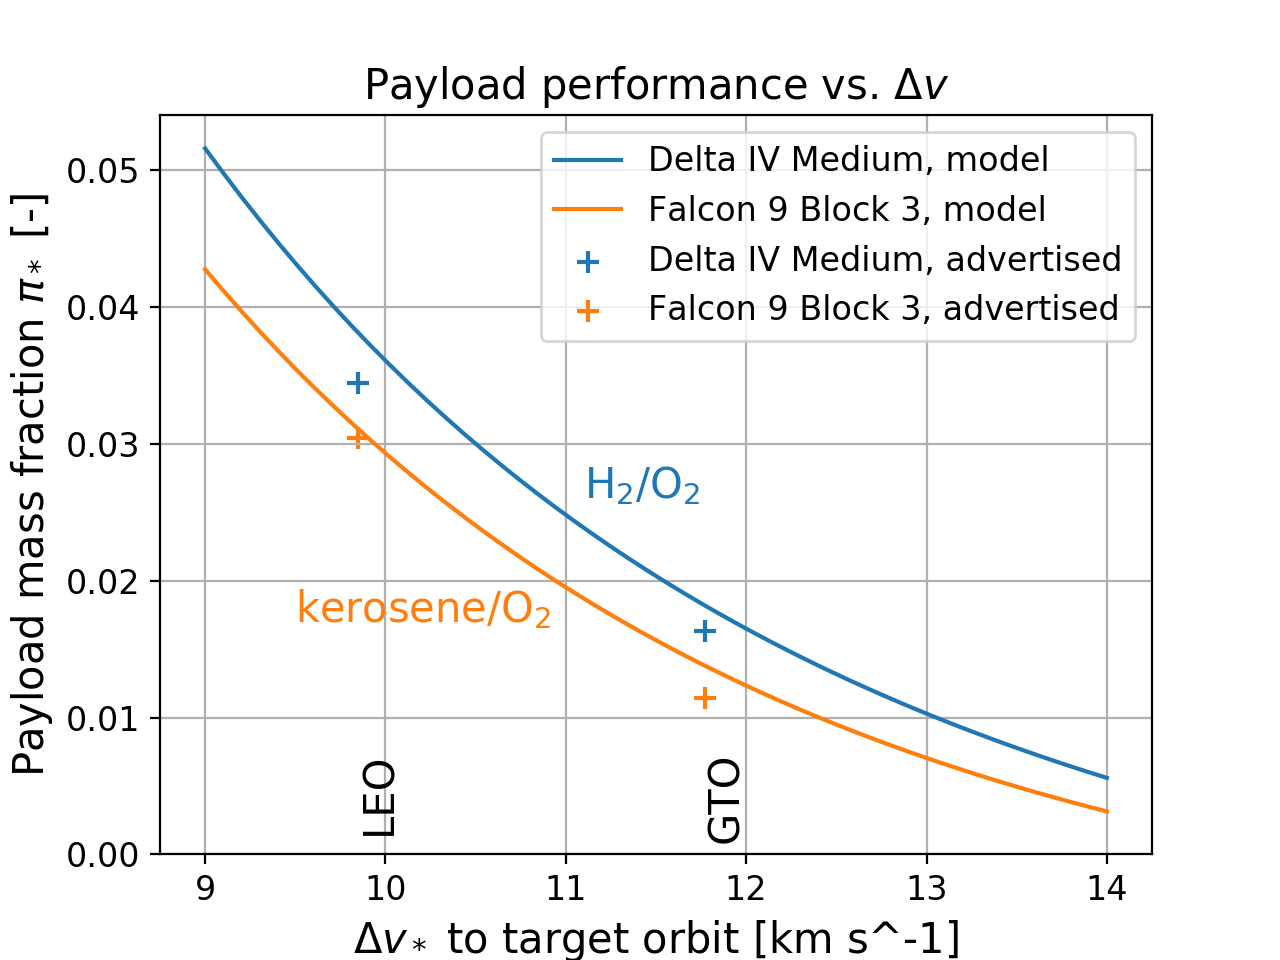
\includegraphics[width=\textwidth]{../../lvreuse/analysis/performance/plots/payload_vs_dv}
    \caption{\label{fig:payload_vs_dv} The quick model makes reasonably accurate predictions of the payload capacity of two expendable launch vehicles. Payload performance declines with increasing $\Delta v_*$, and is slightly higher for \ce{H_2} fueled vehicles than for kerosene vehicles.}
\end{figure}

\subsection{Technology choice}
Clearly, payload performance depends on inert mass fraction and specific impulse, and would be maximized for $\epsilon \rightarrow 0, \quad I_{sp} \rightarrow \infty$. However, there are technological limits on the achievable values, which depend on a collection of design decisions, i.e. the propellant, engine cycle, tank and structure materials, etc. We refer to this collection of decisions as a "technology choice". The technology choice sets $I_{sp, 1}, I_{sp, 2}$, and sets lowers feasible limits for the inert mass fractions, which we will call $E_1, E_2$. The technology choice also influences the cost model (see next section). We will analyze reuse strategies under two example technology choices:

\begin{itemize}
    \item \ce{H2} / \ce{O2} propellants, staged combustion cycle, aluminum alloy tanks
    \item kerosene / \ce{O2} propellants, gas generator cycle, aluminum alloy tanks
\end{itemize}

These technologies are mature and have had fairly consistent specific impulse and inert mass limits over the past 30 years\footnote{This analysis can easily be extended to new technologies, e.g. \ce{CH4} / \ce{O2} propellants or composite tanks, as the engineering limits on these technologies emerge}. Stages using hydrogen technology have higher $I_{sp}$ but higher feasible inert mass $E$ than those using kerosene. The balance of these effects works out to slightly favor hydrogen in terms of payload performance [Figure \ref{fig:payload_vs_dv}]. Finally, note that the technology choice and reuse strategy are independent - any reuse strategy can conceivably be used with any technology choice.


\subsection{How first stage reuse effects performance}
So far we have reviewed the factors determining launch vehicle performance. Now we ask, how does first stage reuse change these factors? Two mechanisms are possible:

\begin{itemize}
    \item \emph{$\Delta v$ losses} - Some reuse strategies require modifying the outer mold line of the stage or altering the ascent trajectory. This changes the drag, gravity and steering losses during ascent, and could cause the $\Delta v_*$ to a target orbit to be different for reusable and expendable strategies.
    \item \emph{Extra mass on the first stage} - All reuse strategies require the first stage to carry some extra mass during ascent, as extra hardware (landing gear, wings, etc.) and/or as propellant reserved for recovery.
\end{itemize}

The first can be ignored, as the variation of losses for different recovery strategies is minor and comparable to the variation in losses for fully expendable vehicles \cite{Stappert2017}. Thus, the main effect of first stage reuse on performance is that extra mass must be carried during ascent.

\subsection{First stage unavailable mass}
We define the "first stage unavailable mass fraction", $\epsilon_1'$, to be the fraction of first stage gross mass that is unavailable to be expelled during ascent, i.e.:

\begin{equation}
\label{eq:epsilon_1_prime}
\epsilon_1' = \frac{m_{inert,1} + m_{pr,1}}{m_{inert,1} + m_{p,1}} = \frac{m_{inert,1} + m_{pr,1}}{m_1}
\end{equation}

where $m_{pr,1}$ is the mass of propellant reserved for recovery maneuvers, and $m_{p,1}$ is the total stage 1 propellant mass.
The payload performance of a vehicle with first stage reuse can be found by substituting $\epsilon_1'$ for $\epsilon_1$ in Equation \ref{eq:dv_2_stage}, and solving Equations \ref{eq:dv_2_stage}-\ref{eq:pi_prod}.

Note that all reuse strategies add unavailable mass to the first stage, so we will always have $\epsilon_1' > E_1$.

The effect of first stage unavailable mass on payload performance is shown in Figure \ref{fig:payload_vs_unavail_mass}. The top plots show the overall payload mass fraction as a function of $\epsilon_1'$. The bottom plots show the payload capacity of a vehicle with first stage reuse as a fraction of the payload capacity of an "equivalent" expendable vehicle with the minimum feasible first stage inert mass fraction $E_1$. Note that the same $\epsilon_1'$ causes a larger fractional reduction of payload capacity on higher $\Delta v$ missions.

\begin{figure}[hbt!]
    \centering
    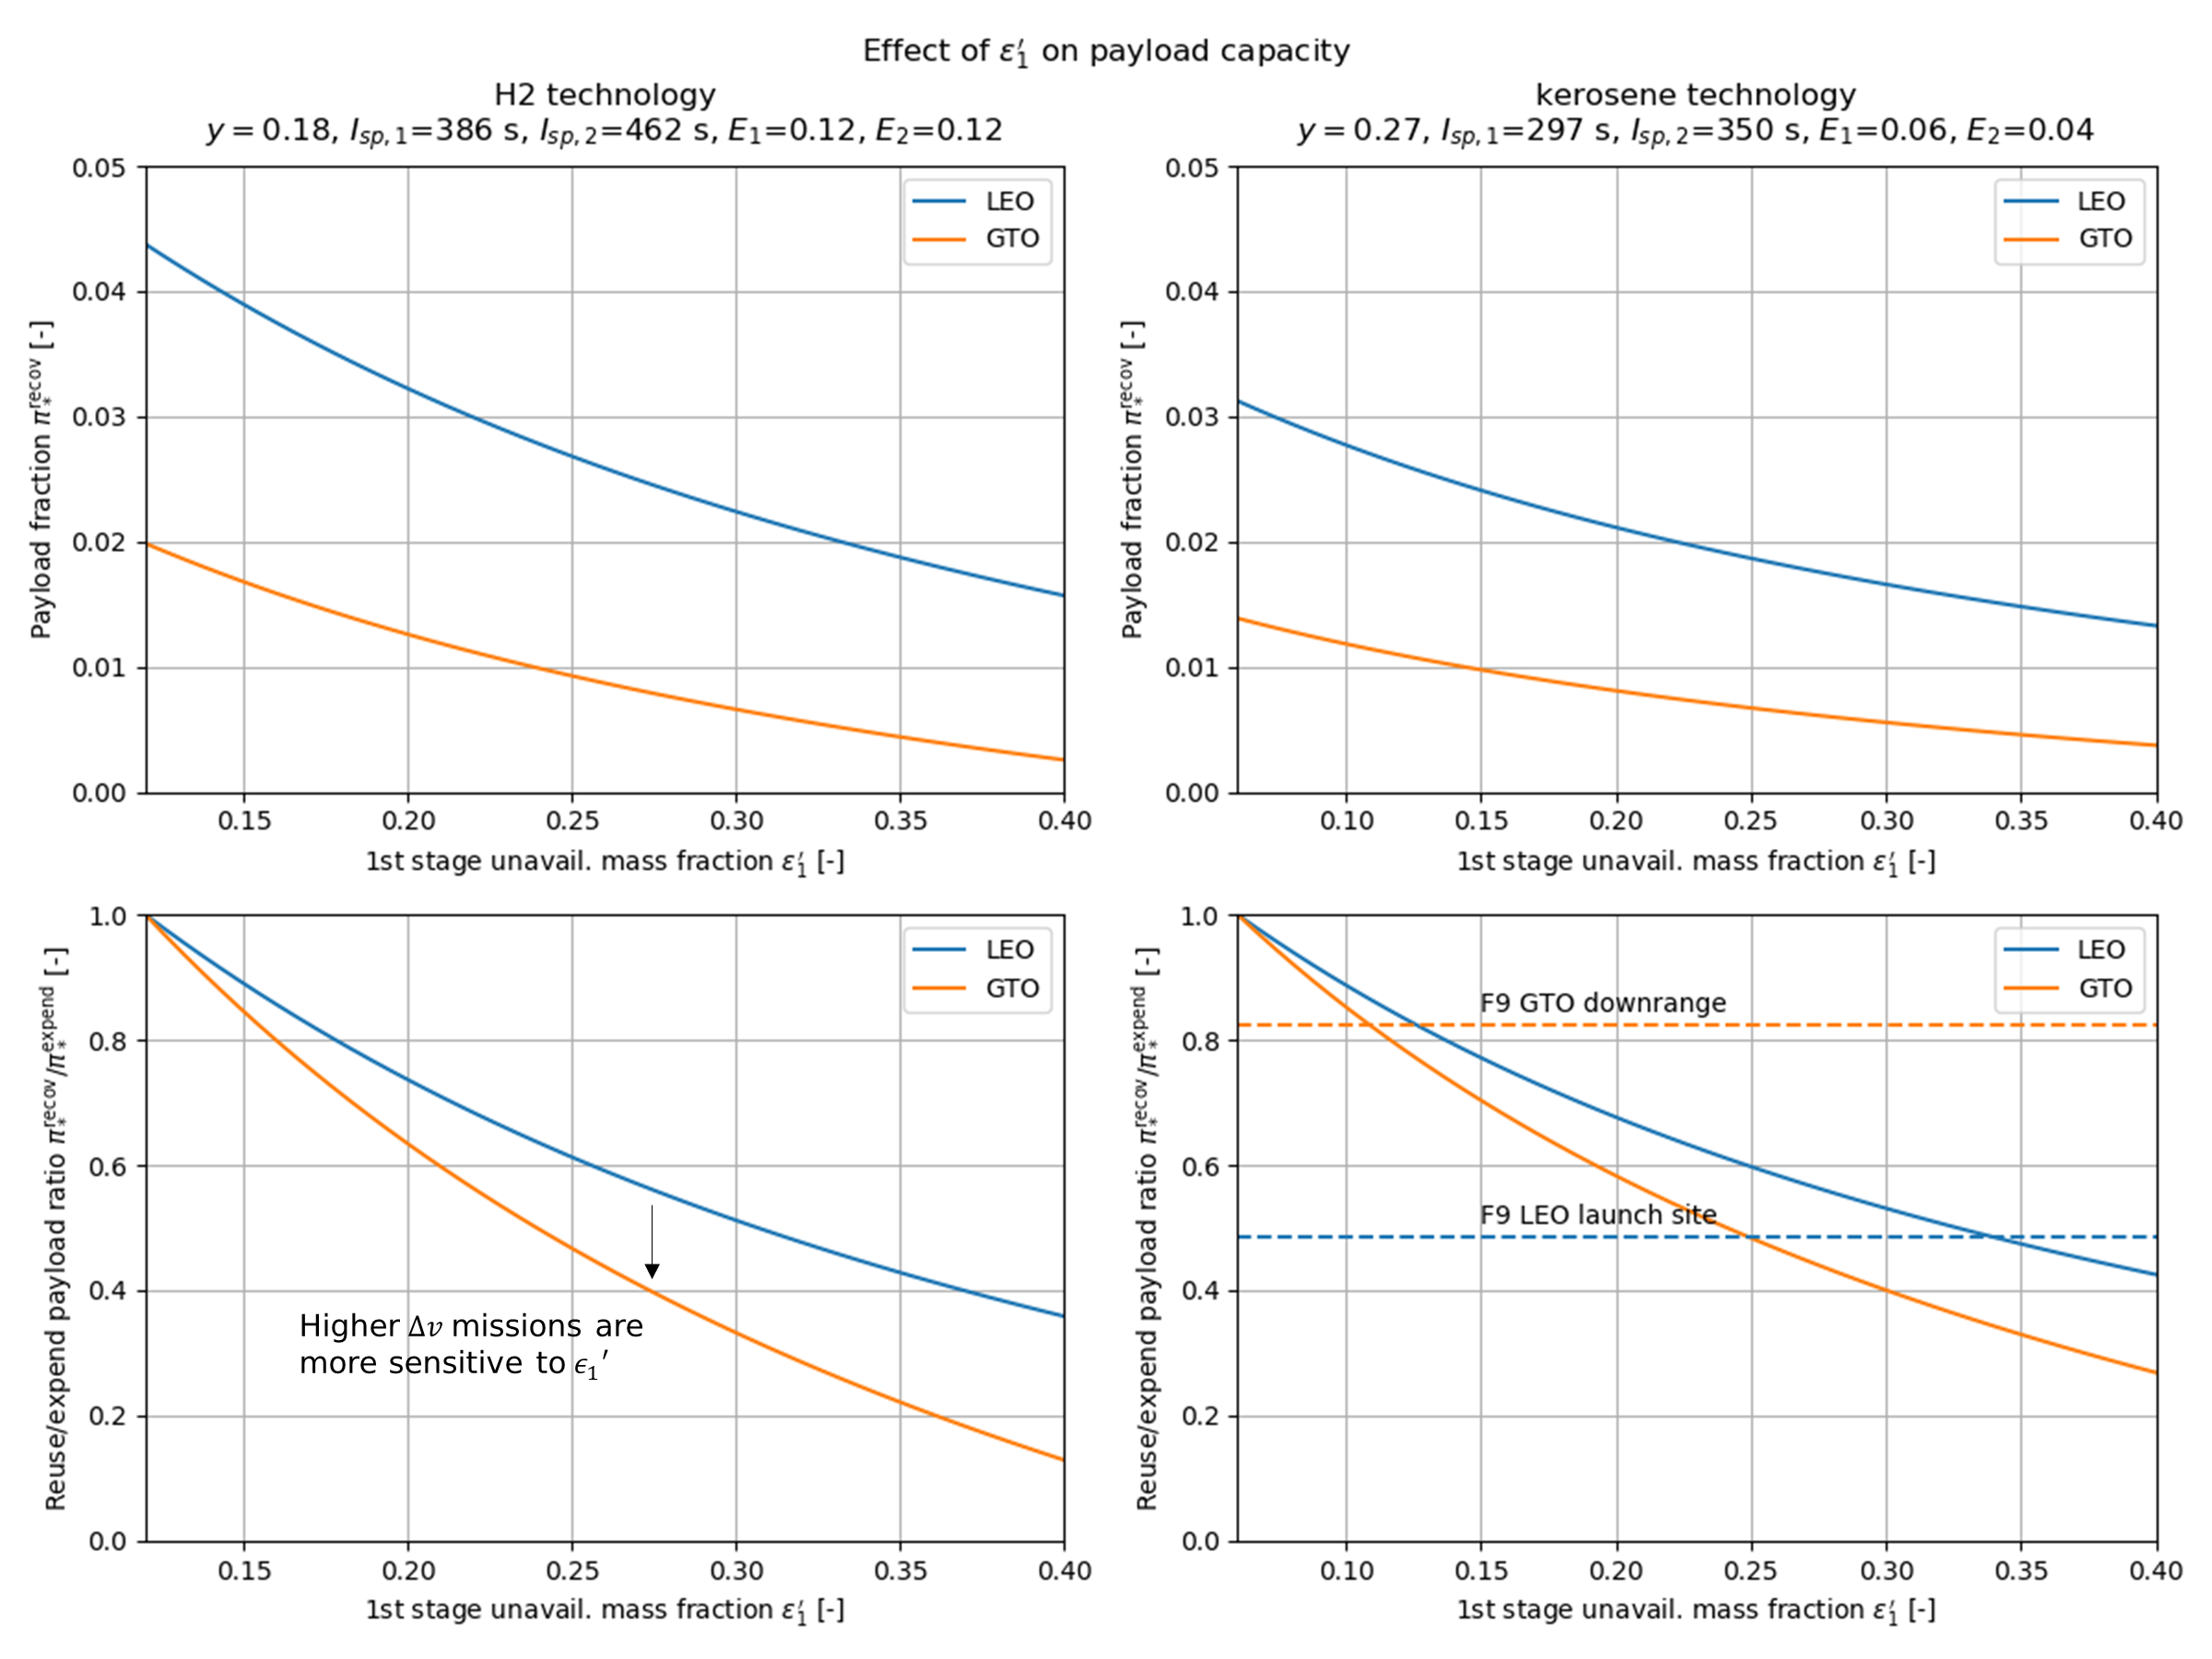
\includegraphics[width=\textwidth]{payload_vs_unavail_mass_annotated}
    \caption{\label{fig:payload_vs_unavail_mass} Payload performance declines as first stage unavailable mass increases.}
\end{figure}

\subsection{Relating unavailable mass to recovery hardware and propulsion}
Next, we relate $\epsilon_1'$ to the feasible limit on inert mass ($E_1$) and the extra hardware and propellant needed for recovery.
It will be helpful to compare the inert mass of the first stage to a "baseline" hardware mass:

\begin{equation}
m_{hb,1} \equiv \frac{E_1}{1 - E_1} m_{p,1}
\end{equation}

i.e. the mass that the first stage would have if it were build to lightest limit feasible for an expendable vehicle. We can think of this as the mass of the baseline hardware that would be present on an expendable first stage, i.e. tanks, rocket engines and thrust structure. In addition to the baseline mass, a reusable stage will have some additional recovery hardware (e.g. wings, landing gear, parachutes) with mass $m_{hr,1}$. Thus, for a reusable stage $m_{inert,1} = m_{hb,1} + m_{hr,1}$.

Then, we define three new dimensionless variables:
\begin{itemize}
    \item $z_m \in (0, 1]$ is the fraction of the first stage baseline mass which is recovered, i.e.
    \begin{equation}
    z_m \equiv \frac{m_{hv,1}}{m_{hb,1}}
    \end{equation}
    where $m_{hv,1}$ is the mass of the valuable hardware to be recovered. For full reuse of the first stage $z_m = 1$. If only an engine pod is recovered, $z_m \approx 0.3$.

    \item $H \in (0, 1)$ is the recovery hardware factor; the mass of the recovery hardware divided by the dry mass of the recovered stage or pod:
    \begin{equation}
    H \equiv \frac{m_{hr,1}}{m_{hr,1} + m_{hv,1}}
    \end{equation}
    The extreme $H=0$ represents the (rather miraculous) situation in which we could recover the valuable hardware without any additional recovery equipment. The extreme $H \rightarrow 1$ represents the situation in which the recovery construction is very poor, and many tons of wings, parachutes, etc. are needed to recover a few kilograms of high-value hardware.

    \item $P \in (0, \infty)$  is the recovery propellant factor. The propellant mass needed for recovery is
    \begin{equation}
    m_{pr,1} = (m_{hr,1} + m_{hv,1}) \left( e^P - 1 \right)
    \end{equation}
    If the recovery maneuvers use rocket propulsion, then $P$ is found from the Tsiolkovsky equation:
    \begin{equation}
    \label{eq:rocket_p}
    P = \frac{\Delta v_r}{g_0 I_{sp,1}}
    \end{equation}
    where $\Delta v_r$ is the $\Delta v$ of the recovery maneuvers. If instead the stage flies back and uses air-breathing propulsion to maintain steady level flight, then $P$ is found from the Berguet range equation:
    \begin{equation}
    \label{eq:berguet_p}
    P =  \frac{R_{\mathrm{cruise}}}{v_{\mathrm{cruise}} (L/D) I_{sp}^{ab}}
    \end{equation}
    where $R_{\mathrm{cruise}}$ is the cruise range, $v_{\mathrm{cruise}}$ is the cruise speed, $(L/D)$ is the cruise lift to drag ratio and $I_{sp}^{ab}$ is the specific impulse of the air breathing engine. If no (mass-expelling) propulsion is used during recovery, $P = 0$ and $m_{pr,1} = 0$.
\end{itemize}

It can be shown that (see appendix TODO):

\begin{equation}
\label{eq:eps_h_p_z}
\epsilon_1' = \frac{1 + \frac{H z_m}{1 - H} +  \frac{z_m}{1 - H} (e^P - 1) }{1 + \frac{H z_m}{1 - H} + \frac{1 - E_1}{E_1} }
\end{equation}

For full recovery ($z_m = 1$) this simplifies to:
\begin{equation}
\epsilon_1' = \frac{e^P}{1 + (1 - H) \left( \frac{1 - E_1}{E_1} \right)}
\end{equation}

Note that $\epsilon_1'$ increases monotonically with $z_m, H$ and $P$; i.e. recovering more of the stage, using more recovery hardware or using more recovery propellant all increase the unavailable mass.

Now, we can estimate the unavailable mass of the first stage (and therefore the launch vehicle payload performance) from the portion of the stage recovered ($z_m$) and estimates of the hardware ($H$) and propulsion ($P$) required by the selected recovery strategy. 

\subsection{Estimating hardware and propulsion for recovery strategies}
In this subsection, we establish estimates of the recovery hardware factor $H$ and propellant factor $P$ for various recovery strategies.

We account for uncertainty in our model using Monte Carlo techniques. In a preliminary design we do not know enough details to make point estimates of $H$, $P$ and the other model input parameters. Instead, we estimate the credible range that each the model input parameter could lie in, and fit probability distributions to these estimates. We then draw many random samples from the input distribution and evaluate our model on each sample to generate a population of model outputs. This population then represents the range of values that the model output can be expected to take on.

A brief summary of the input parameter distributions is given below; more detail is given in appendix TODO.

We estimate $H$ by examining the mass breakdowns of detailed design studies for some types of reusable boosters \cite{Healy1998, Isakowitz2004, Sippel2003, Hellman2005}, and by analogy to the mass breakdowns of other aerospace vehicles. The resulting estimates are summarized in Table \ref{tab:hardware_factor_distributions}.

\begin{table}[hbt!]
    \centering
    \caption{\label{tab:hardware_factor_distributions} Uncertainty distribution parameters of the recovery hardware factor $H$. $H$ can run from 0 to 1, higher values of $H$ indicate that more recovery hardware is needed.}
    \begin{tabular}{l l c c c}
    \hline
     & \multicolumn{3}{c}{Triangular dist. params.} \\
     & Min & Mode & Max \\
    \hline
    \hline
    Winged, Glider  & 0.380 & 0.426 & 0.540 \\
    Winged, Air-breathing & 0.490 & 0.574 & 0.650 \\
    \hline
    Propulsive landing  & 0.09 & 0.14 & 0.19 \\
    \hline
    Parachutes & 0.050 & 0.065 & 0.080 \\
    Parachutes and inflatable heat shield  & 0.150 & 0.170 & 0.190 \\
    \hline
    \end{tabular}
\end{table}

We do not estimate $P$ directly; rather we assume distributions on the factors determining $P$. For propulsive landing, these are the $\Delta v$ of the entry burn (which could be \SIrange{0}{1000}{\meter\per\second}), and the $\Delta v$ of the landing burn (which depends on the stage's ballistic coefficient and the landing burn acceleration) [Figure \ref{fig:propulsive_landing}]. For winged stages with air-breathing propulsion, these factors are the lift/drag ratio (4 to 8), air breathing engine specific impulse (\SIrange{3200}{4000}{\second}), and cruise speed (\SIrange{100}{300}{\meter\per\second}) during the powered cruise portion of the return trajectory [Figure \ref{fig:flyback_trajectory}].

For launch site recovery there is a further wrinkle - the stage separation velocity $v_{ss}$ depends on the unavailable mass ($v_ss$ decreases as $\epsilon_1'$ increases). But for return-to-launch-site strategies, the recovery propellant factor $P$ (and therefore $\epsilon_1'$) depends on $v_{ss}$. Thus, for return-to-launch-site strategies, we solve simultaneously for $\pi_*, \epsilon_1'$ and $P$. For rocket propelled return, we compute the impulsive $\Delta v$ needed to place the stage on a ballistic trajectory to the launch site, plus gravity losses. For air-breathing return, we use the Berguet range equation \footnote{In both cases, we model the downrange distance at stage separation as $R = f_{ss} v_{ss}^2$, where $f_{ss}$ is an uncertain coefficient, whose dispersion is calibrated to data from actual launches and detailed trajectory simulations}.

The specific impulses and minimum feasible inert mass fractions are also dispersed. Their distributions are based on data from previous launch vehicles and engines \cite{Isakowitz2004, hist_lpre}. 

% TODO do we really need these figures here?
\begin{figure}[hbt!]
    \centering
    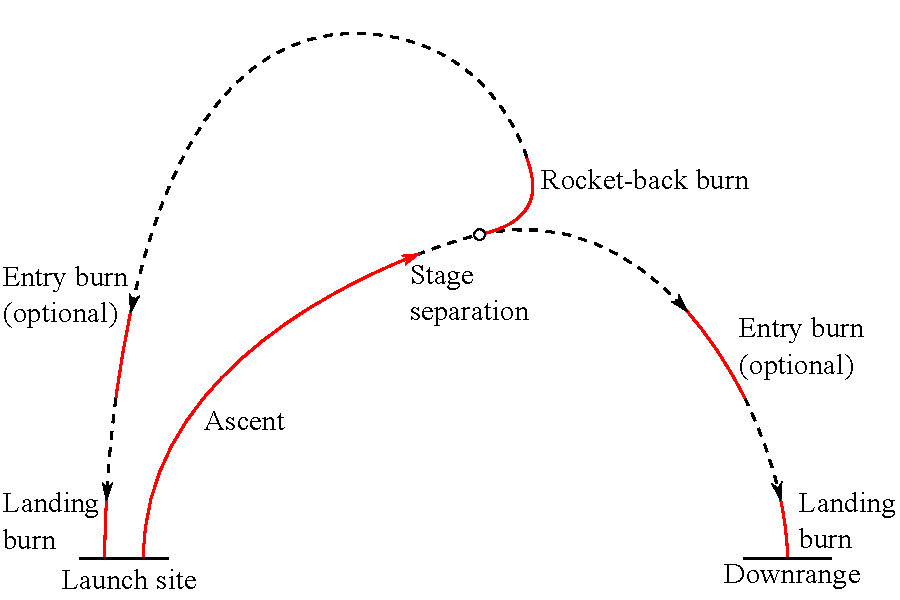
\includegraphics[width=0.5\textwidth]{propulsive_landing}
    \caption{\label{fig:propulsive_landing} Propulsive landing: trajectory options for launch site and downrange recovery. Propulsive portions of the trajectory are shown as red solid lines.}
\end{figure}


\begin{figure}[hbt!]
    \centering
    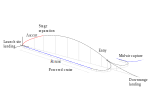
\includegraphics[width=0.7\textwidth]{flyback_trajectory}
    \caption{\label{fig:flyback_trajectory} Winged landing: trajectory options for launch site and downrange recovery. Portions of the trajectory flown under rocket propulsion are shown as red solid lines; air-breathing propulsion is indicated with blue.}
\end{figure}

These estimates are summarized in Figure \ref{fig:unavail_mass_contours}, which shows contours of $\epsilon_1'$ on $P$ vs. $H$ axes. The likely ranges of $P$ and $H$ for some recovery strategies are shown as blue ellipses. This figure assumes kerosene technology and full recovery of the first stage. Note that the (launch site, rocket-propelled, propulsive landing) strategy incurs the highest unavailable mass because of the large amount of propellant required to return the stage to the launch site. The (downrange, no propulsion, parachute landing) strategy has the lowest unavailable mass. 

\begin{figure}[hbt!]
    \centering
    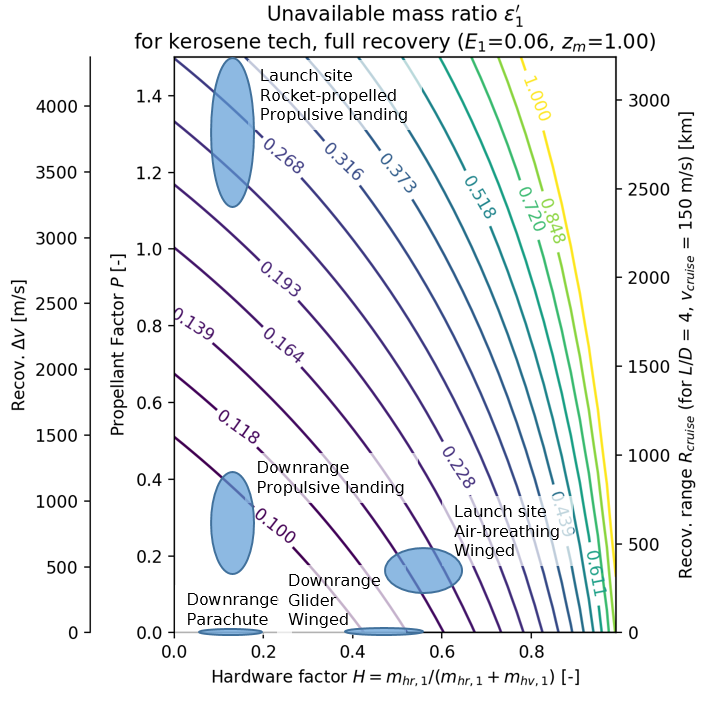
\includegraphics[width=0.7\textwidth]{unavail_mass_contours_annotated}
    \caption{\label{fig:unavail_mass_contours} Contours of unavailable mass versus the recovery propellant and hardware factors. Credible ranges for some recovery strategies are shown.}
\end{figure}


\subsection{Payload fraction estimates for recovery strategies}
The distributions of payload performance resulting from this model are shown as violin plots in Figures \ref{fig:strategy_perf_kerosene} and \ref{fig:strategy_perf_H2}. A different plot is provided for each combination of technology choice (kerosene, \ce{H2}) and mission (LEO, GTO). First, note the spread of the distribution for a fully expendable vehicle - this indicates the uncertainty due to technology factors ($I_{sp}$ and $E$). We should only consider a reuse strategy to have a meaningful impact on payload performance if most of its $\pi_*$ distribution does not overlap the range of $\pi_*$ that can be expected from an expendable vehicle.

Across all technology choices and missions, the parachute landing strategies have little impact on payload performance, and their difference from the expendable performance is small compared to the range of uncertainty. The (launch site, air-breathing, winged, partial recovery), (downrange, propulsive landing, full recovery), and (downrange, no propulsion, winged, full recovery)  strategies have slightly lower payload performance than expendable, and are almost indistinguishable from each other.  Propulsive landing at the launch site has the worst payload performance; with kerosene on a GTO mission its payload mass fraction is unacceptably low. Across all strategies, reuse causes a larger fractional decrease in $\pi_*$ on the higher-$\Delta v$ mission (GTO).

These payload mass fraction estimates allow us to predict the mass of the launch vehicle required to lift a payload into a target orbit. In the next section, we develop a model that uses the launch vehicle masses, along with other factors, to estimate system cost.

\begin{figure}[hbt!]
    \centering
    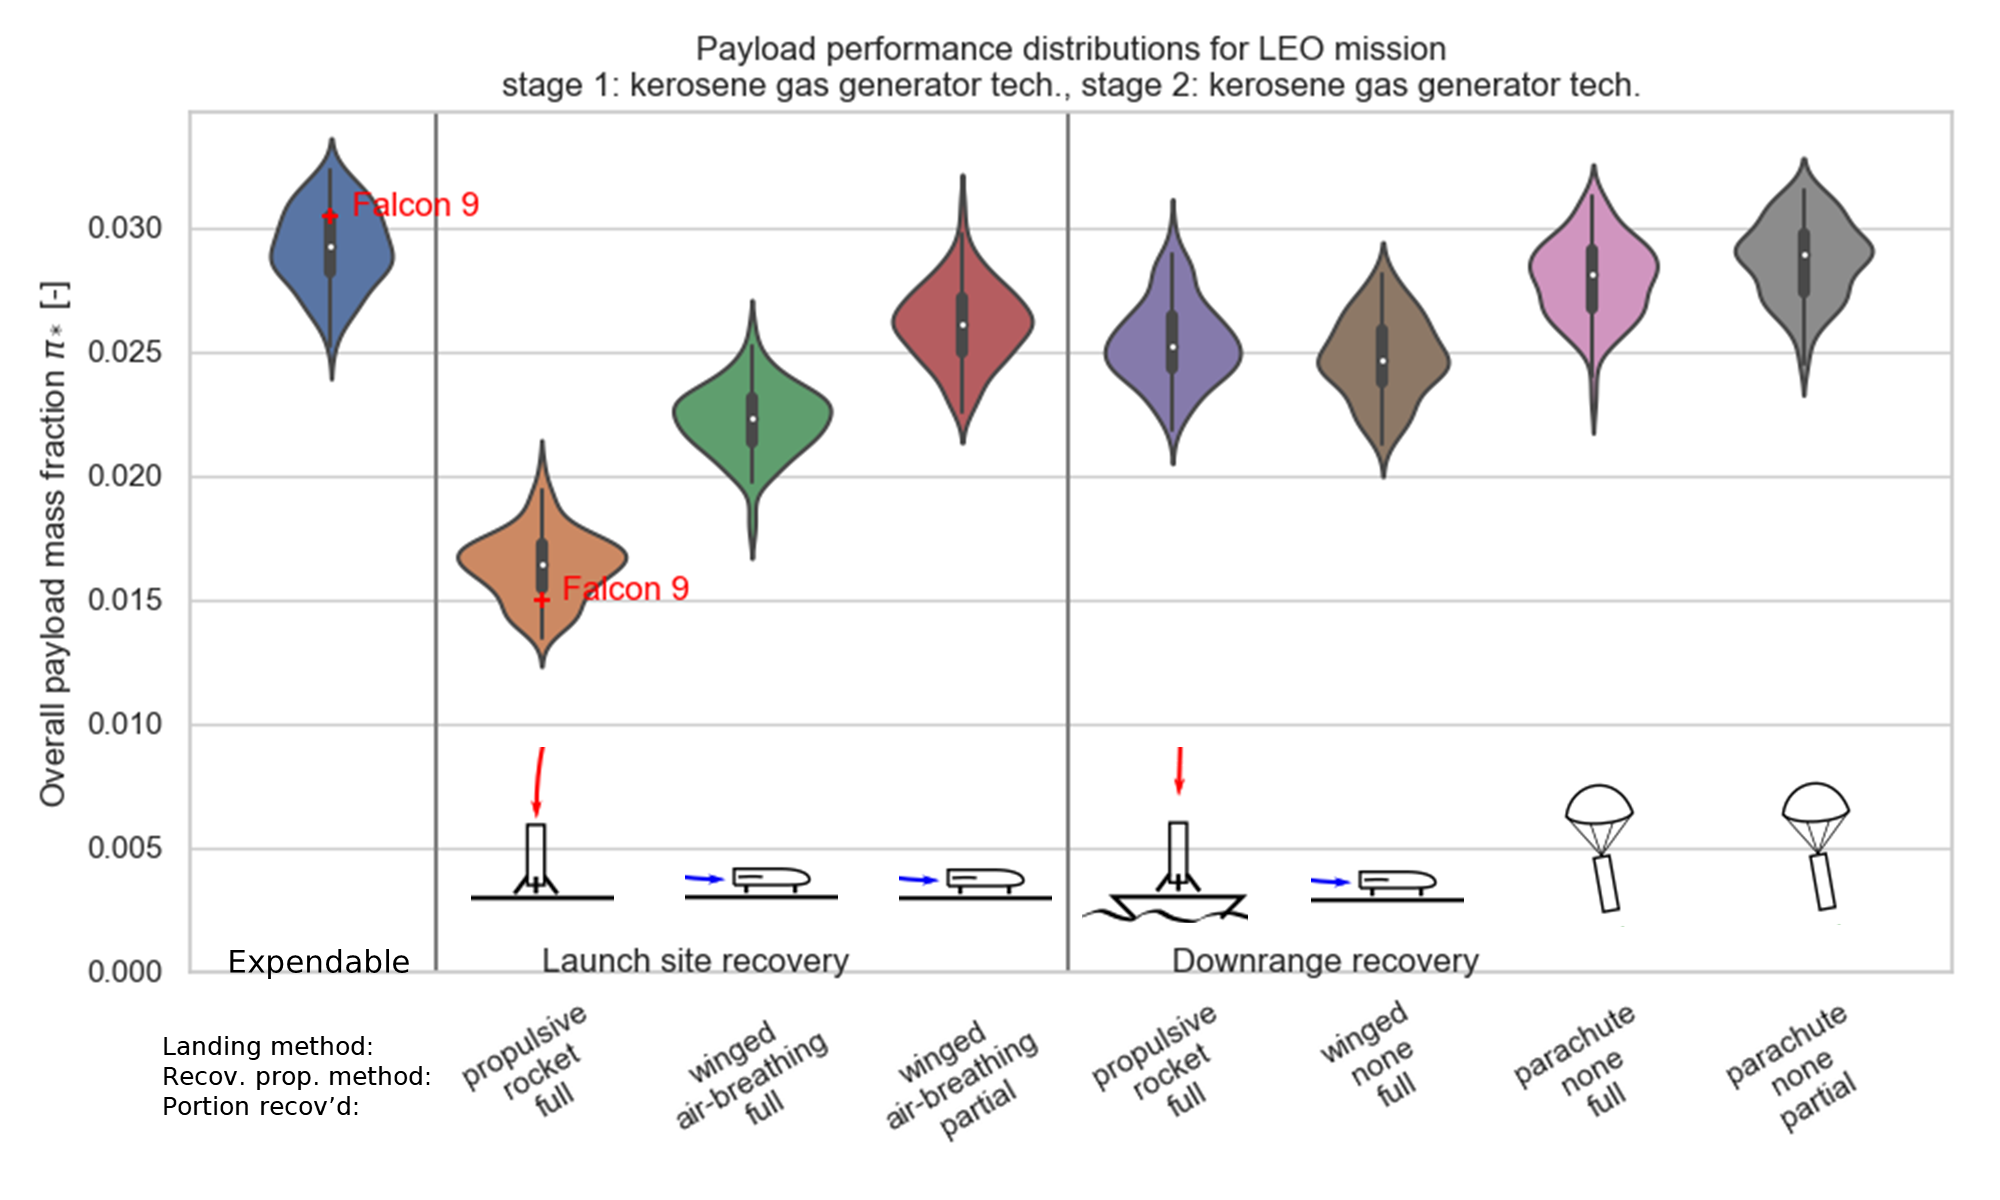
\includegraphics[width=\textwidth]{strategy_perf_annotated/LEO_kero}
    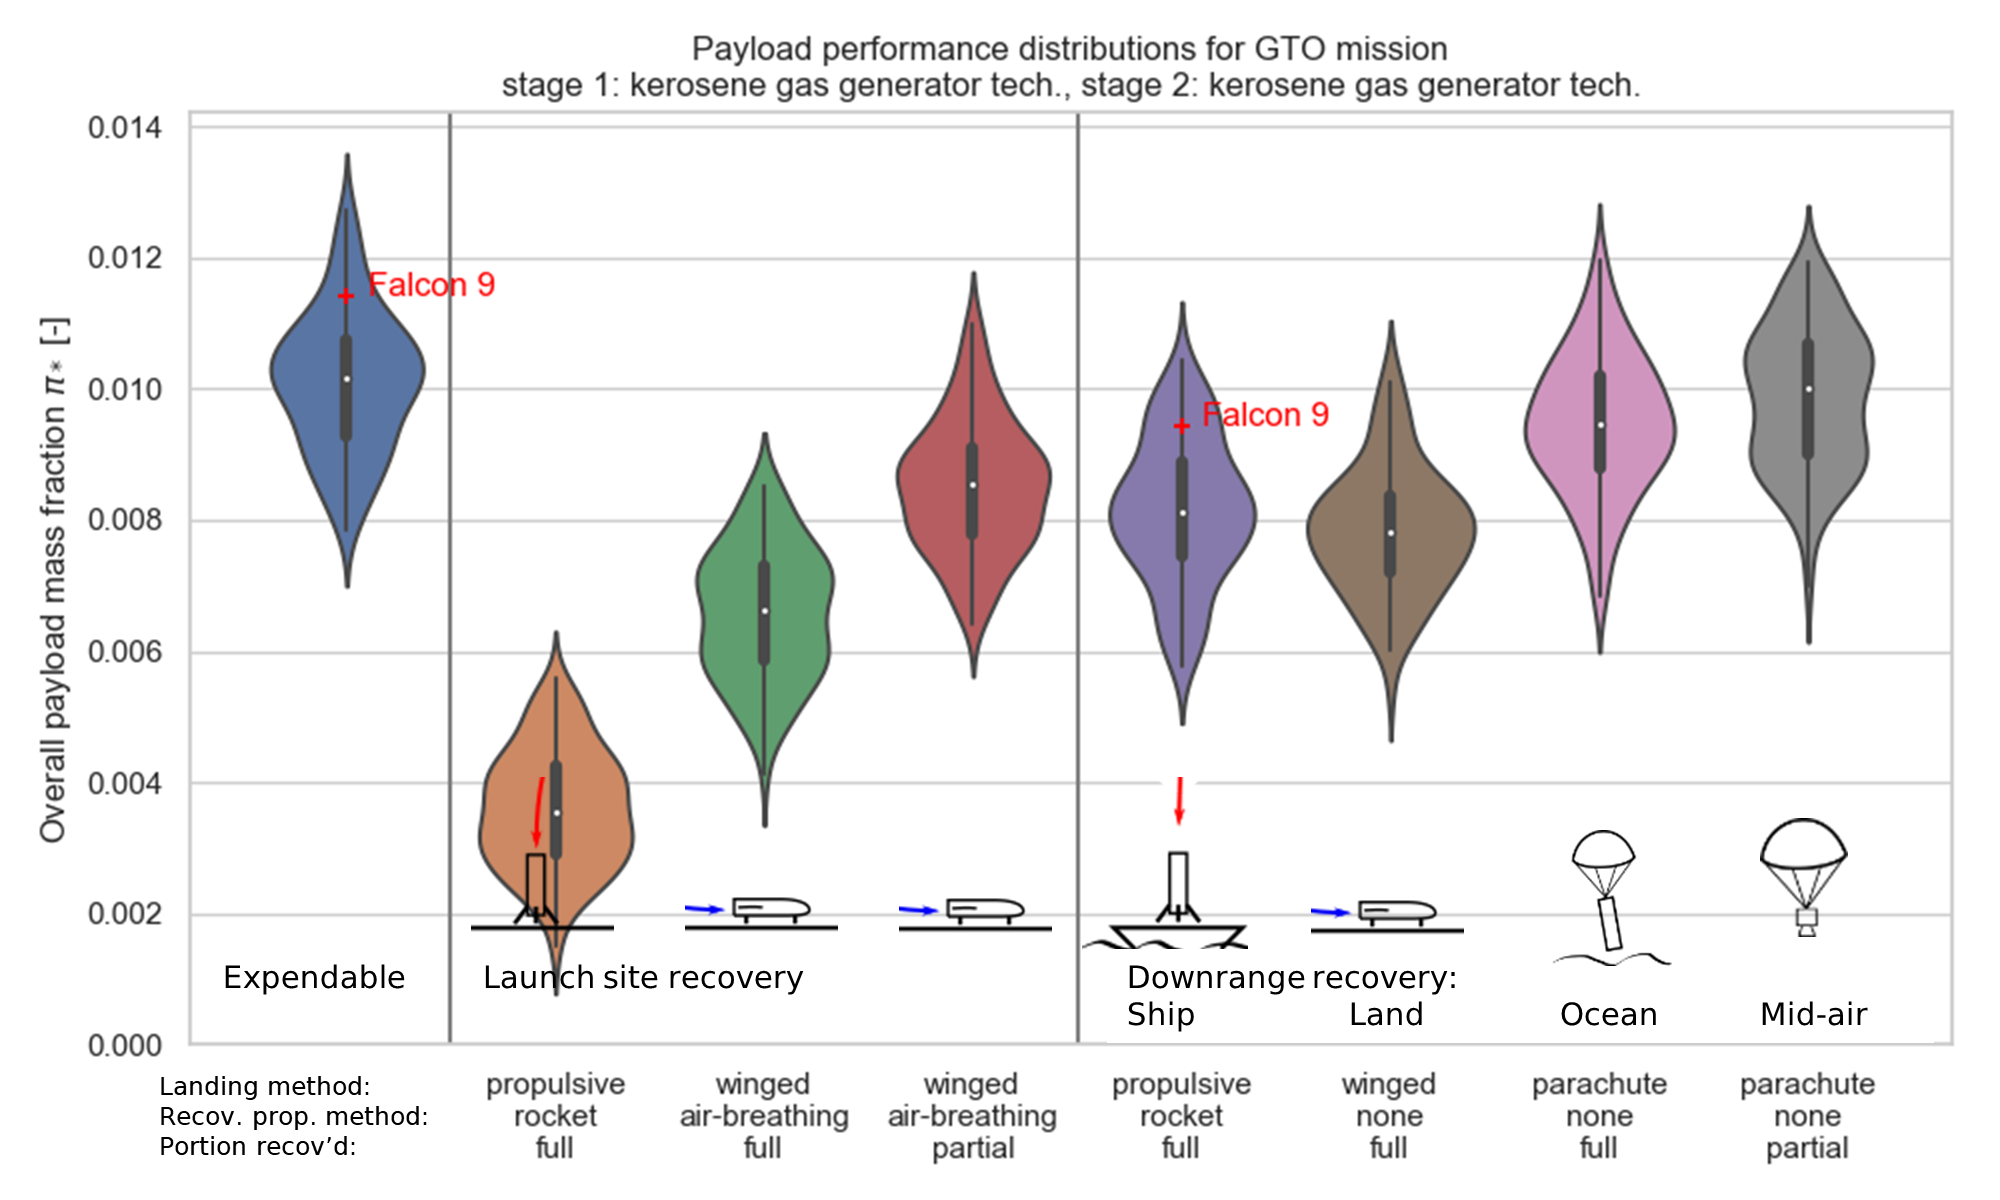
\includegraphics[width=\textwidth]{strategy_perf_annotated/GTO_kero}
    \caption{\label{fig:strategy_perf_kerosene} Distributions of payload performance for various first stage recovery strategies with kerosene technology. Reported payload performance for Falcon 9 block 3 is shown for comparison.}
\end{figure}

\begin{figure}[hbt!]
    \centering
    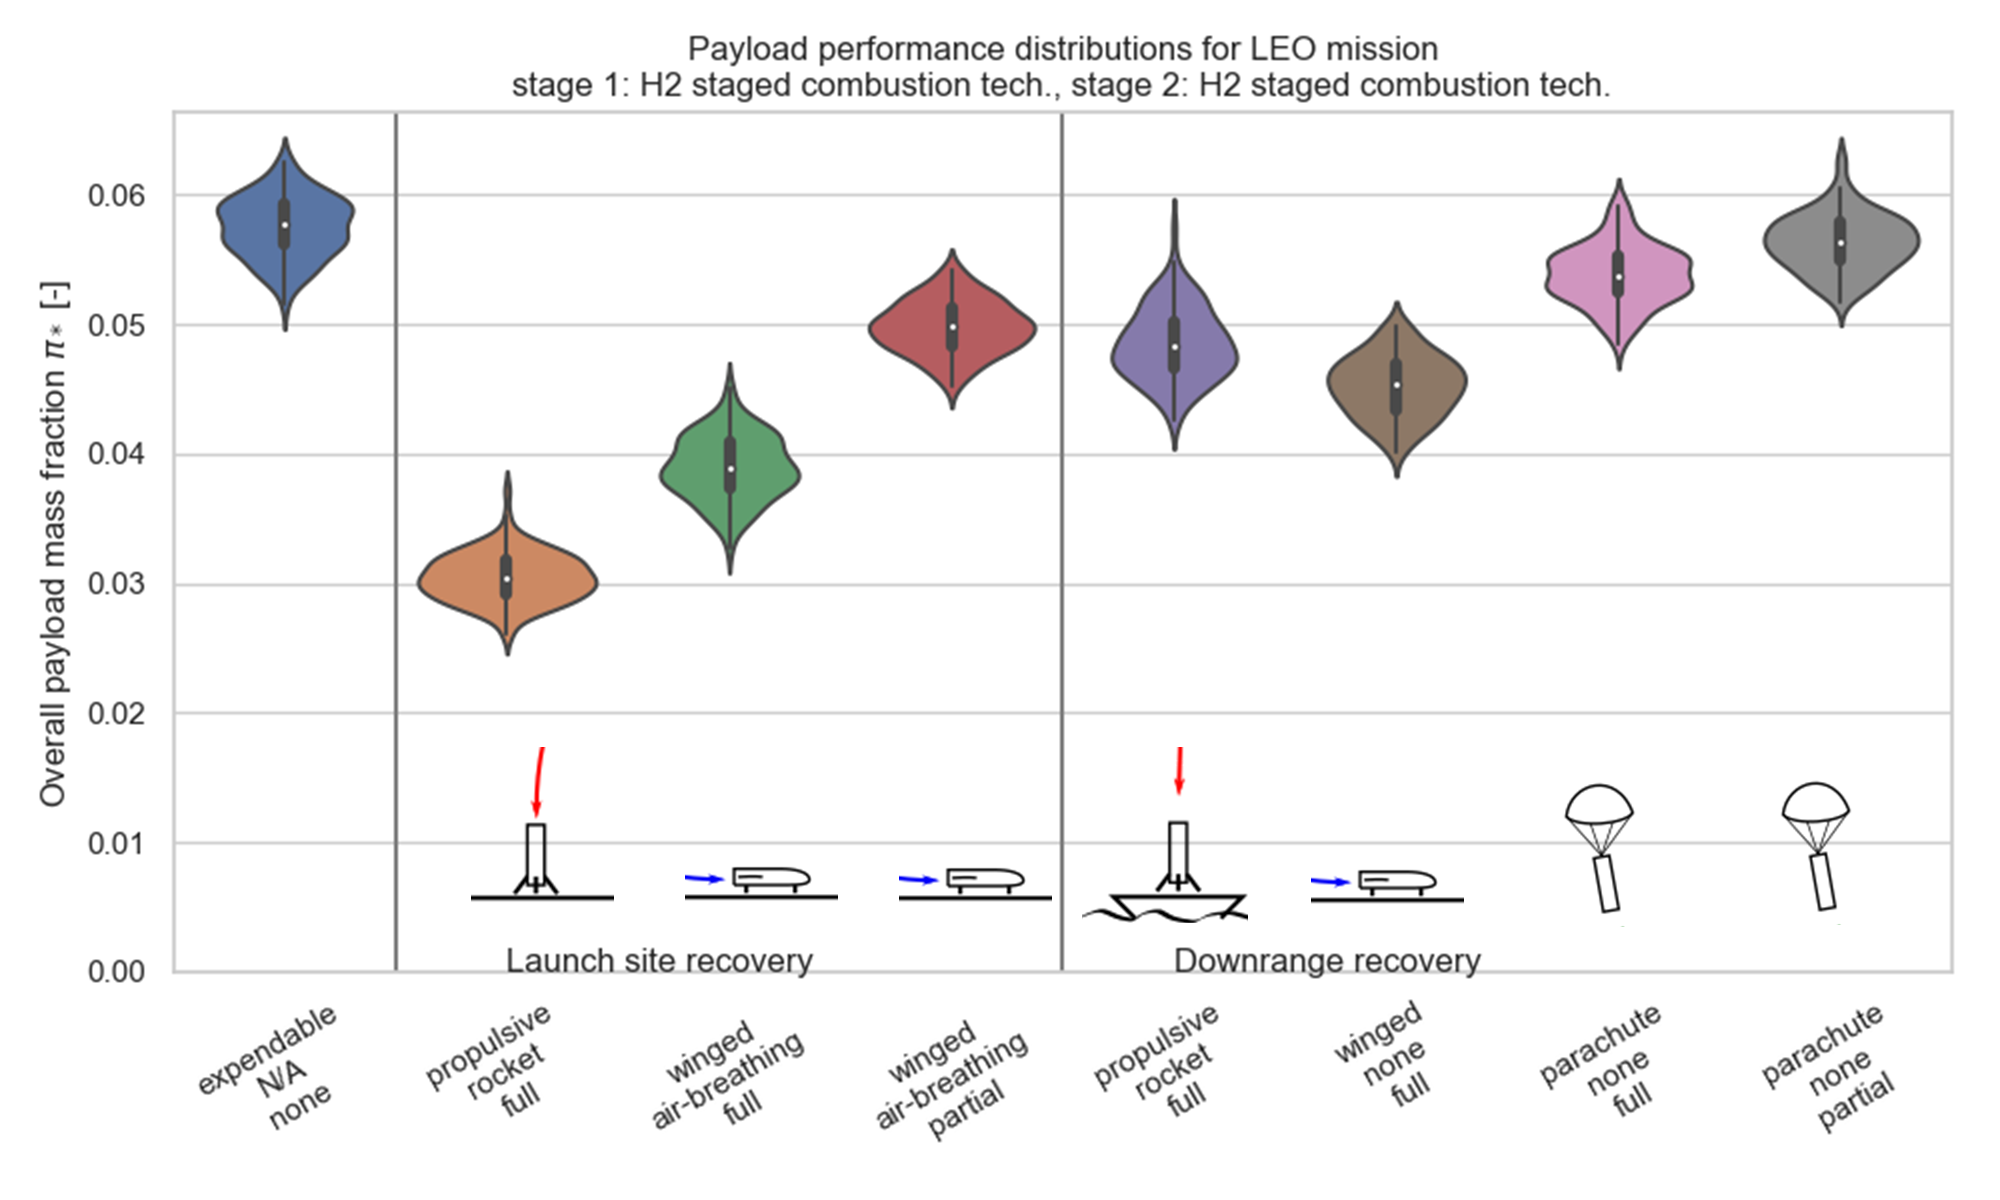
\includegraphics[width=\textwidth]{strategy_perf_annotated/LEO_H2}
    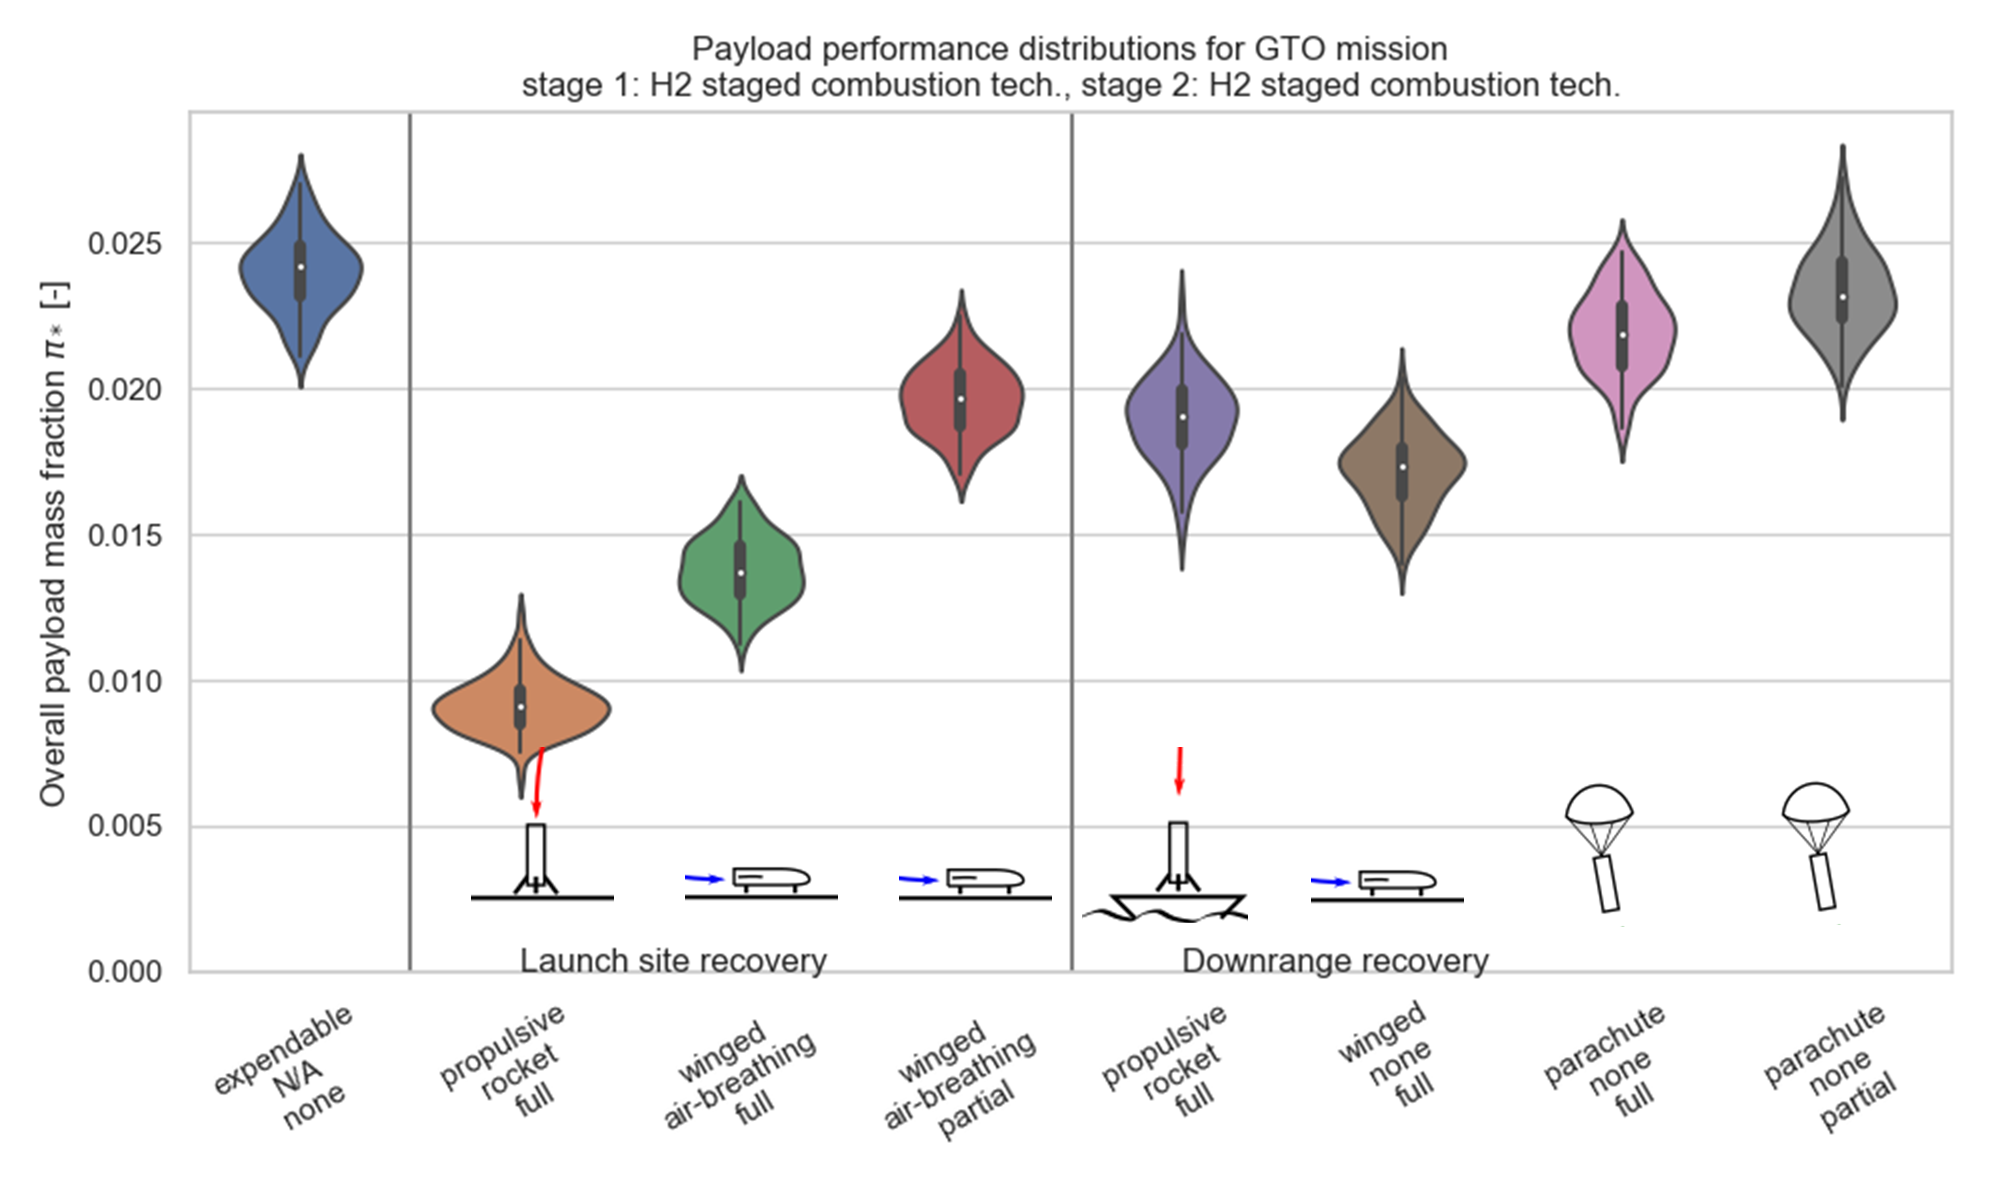
\includegraphics[width=\textwidth]{strategy_perf_annotated/GTO_H2}
    \caption{\label{fig:strategy_perf_H2} Distributions of payload performance for various first stage recovery strategies with \ce{H2} technology.}
\end{figure}

\bibliography{first_stage_recovery}

\end{document}